\renewcommand{\theequation}{\theenumi}
\renewcommand{\thefigure}{\theenumi}
\renewcommand{\thetable}{\theenumi}
\begin{enumerate}[label=\thesection.\arabic*.,ref=\thesection.\theenumi]
\numberwithin{equation}{enumi}
\numberwithin{figure}{enumi}
\numberwithin{table}{enumi}

\item Let $X$ be a Poisson random variable with p.m.f
\begin{align}
\label{poisson/1/eq:1}
P(X=k) = 
    \begin{cases} 
      \frac{e^{-\lambda}\lambda^{k}}{k!},& k=0,1,2,...;  \lambda > 0\\
      0 & \text{otherwise}
   \end{cases}
\end{align}
If $Y = X^2 + 3$, then what is $P(Y=y)$ equal to?
\begin{enumerate}[label={(\Alph*)}]
    \item $\frac{e^{-\lambda}\lambda^{\sqrt{y-3}}}{\sqrt{\brak{y-3}}!}$, for $y =$ \cbrak{3,4,7,12,...}
    \item $\frac{e^{-\lambda}\lambda^{-\sqrt{y-3}}}{\sqrt{\brak{3-y}}!}$, for $y =$ \cbrak{3,4,7,12,...}
    \item $\frac{e^{-\lambda}\lambda^{\sqrt{3-y}}}{\sqrt{\brak{3-y}}!}$, for $y =$ \cbrak{4,7,12,...}
    \item $\frac{e^{-\lambda}\lambda^{-\sqrt{3-y}}}{\sqrt{\brak{3-y}}!}$, for $y =$ \cbrak{4,7,12,...}
\end{enumerate}
%
\solution
%
\begin{align}
    Y = X^2 + 3\\
\implies     X = \sqrt{Y - 3}
\end{align}
Substituting $k = \sqrt{y-3}$ in \eqref{poisson/1/eq:1},
\begin{align}
p_Y(y) = 
    \begin{cases} 
      \frac{e^{-\lambda}\lambda^{\sqrt{y-3}}}{\sqrt{\brak{y-3}}!}, & y=3,4,7,12,...\\
      0&\text{otherwise}
   \end{cases}
\end{align}
Hence, the correct option is \brak{A}.
\begin{figure}[hb]
    \centering
    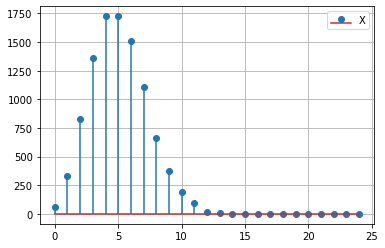
\includegraphics[width=\columnwidth]{poisson/solutions/1/Figures/FigureX.png}
    \caption{Poisson stem plot for X \brak{\lambda = 5}}
    \label{poisson/1/fig:plot1}
\end{figure}
\begin{figure}[hb]
    \centering
    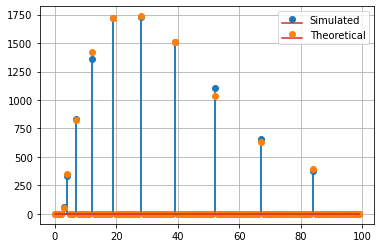
\includegraphics[width=\columnwidth]{poisson/solutions/1/Figures/FigureComp.png}
    \caption{Stem plot for Y (Simulated and Theoretical) \brak{\lambda = 5}}
    \label{poisson/1/fig:plot3}
\end{figure}




\end{enumerate}